\section{Experiment 1: Pre-exposure ratings}
\label{sec:exp-norming}

We first conducted a norming study, which served the following theoretical and methodological purposes.
First, it served as a methodological check on whether the paradigm is suited for 
manipulating fine-grained event probabilities. 
Second, it addressed the theoretical question of whether listeners vary in their expectations about
a generic speaker's use of uncertainty expressions, by collecting participants' judgments about 
uncertainty expressions they expected speakers to use for varying probabilities of receiving gumballs of a particular color from a gumball machine. 
Third,  the results from this study informed the experimental design of the adaptation experiments 
reported in later sections, by allowing us to both choose which pair of uncertainty expressions to test adaptation on, 
and to determine the particular event probability for which participants had roughly equi-probable expectations 
about which expression of uncertainty a generic speaker would use to report an event with that probability. 
Lastly, we used the data collected in this study to 
estimate population-level prior beliefs for the adaptation model reported in Section 5.

\subsection{Method}

\subsubsection{Participants}
We recruited a total of 420 participants 
(20 per condition) on Amazon Mechanical Turk. 
We required participants to have a US-based IP address and a minimal approval rating of 95\%.
Participants were paid \$1.80 (condition 1), \$1.50 (conditions 2-15),
or \$2.00 (conditions 16-21),
depending on the number of trials,
which amounted to an hourly wage of approximately \$12--\$15. 


% Figure 2: plots/fig-2-pre-test-example-trial.jpg (one column figure)
\begin{figure}[th!]
\center
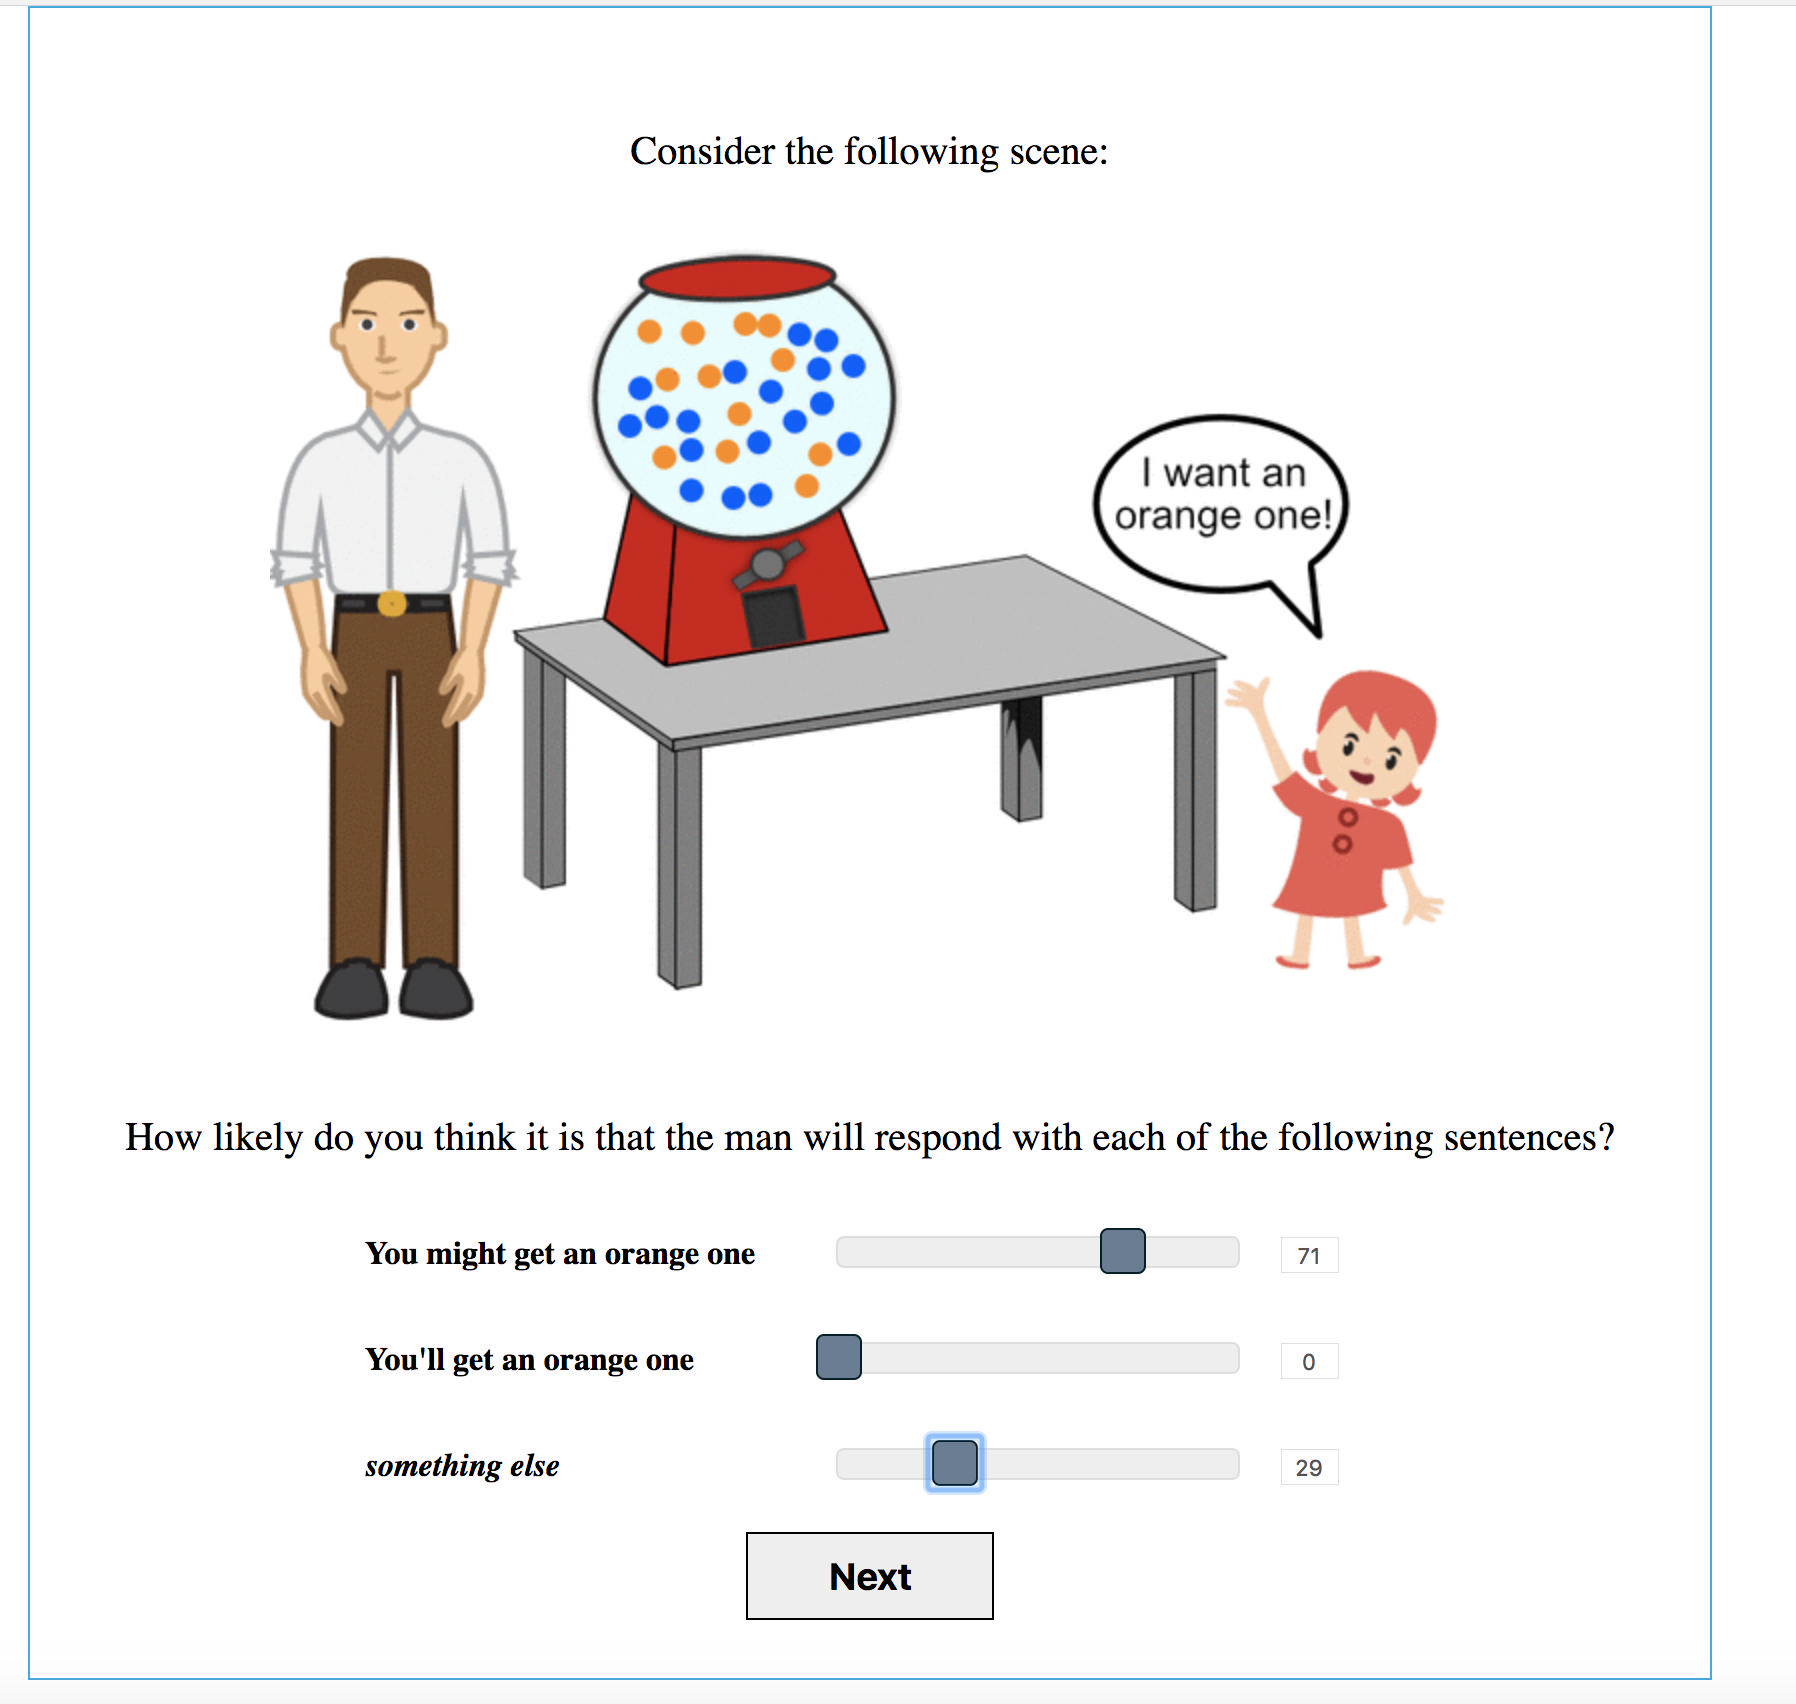
\includegraphics[width=0.7\textwidth, trim={0 0 1.1cm 0},clip]{plots/fig-2-pre-test-example-trial.jpg} 
\caption{Example trial in Experiment~1. \label{fig:norming-trial} }
\end{figure}

\subsubsection{Materials and Procedure}
This study was a production expectation experiment intended to probe listeners' expectations about a generic speaker's language use.
Participants were instructed that over the course of the experiment, they would see several scenes with an adult man, 
a young girl, and a gumball machine on a table and 
that the gumball machine is too high up on the table for the girl to see (see Figure~\ref{fig:norming-trial} for an example scene). 
After completing an attention check which asked participants whether 
the girl could see the gumball machine,\footnote{Participants had to go back to the instructions in case they responded incorrectly. This was the case for 41 participants.} 
participants saw a series of scenes  and were asked to rate how likely they thought it was that the 
adult would produce two given responses by distributing 100 points across the two given utterances and the 
blanket \textit{something else} option (\textsc{other}). Sliders automatically jumped back if participants tried to distribute more than 100 points. 
In each scene, the child uttered \textit{``I want a blue one''} (target color: blue) or  \textit{``I want an orange one''} (target color: orange), randomized across participants.\footnote{In condition 1 (\textit{bare-might}), as well as conditions 16-21 (all conditions with \textit{bare not}), the target color was randomized across trials. While randomization of the target color across trials increased the correlation between the ratings for the two colors,  the average ratings for each condition independent of the target color were not affected by this choice. See Appendix A or a detailed discussion of the effect of this manipulation on the ratings.} The gumballs in the machines were tossed around continuously to prevent participants from counting the gumballs
and to make sure that participants did not consider it more likely to get one of the gumballs at the bottom of the machine.
 In each of the 21 conditions, participants saw only  two of the following seven possible adult utterances with different uncertainty expressions:\footnote{In the choice of the investigated expressions, we follow recent work on the interpretation of uncertainty expressions \cite{Pogue2018} and aim to use naturalistic utterances. We therefore decided against using a frame such as \emph{``It is UNCERTAINTY-ADJ that''} that would have fixed the syntactic structure across items because such a frame would have resulted in less naturalistic expressions like  \emph{``It is possible that''} or  \emph{``It is probable that''}, which are much less common than the expressions we considered (e.g., \textit{might} appears more than 30 times more often than \textit{possible that} in the spoken portion of the Contemporary American English \cite{Davies2009}). A speaker's use of these rare expressions thus could have triggered additional pragmatic inferences due to violations of the maxim of manner \cite{Grice1975} that are unrelated to our research questions.}

 \begin{itemize}
\item You'll get a blue/orange one. (\textsc{bare}\footnote{As a notational convention, we refer to utterances with uncertainty expressions in \textsc{small caps} and to the uncertainty expression itself in \textit{italics}. })
\item You might get a blue/orange one. (\textsc{might})
\item You'll probably get a blue/orange one. (\textsc{probably})
\item I think you'll get a blue/orange one. (\textsc{think})
\item It looks like you'll get a blue/orange one. (\textsc{looks like})
\item You could get a blue/orange one. (\textsc{could})
\item You won't get a blue/orange one. (\textsc{bare not})
\end{itemize}


\noindent Within each condition, we manipulated the percentage of target color gumballs across trials, which we take as proxy for the objective probability of receiving a gumball of the target color. 
Each participant saw 3 trials\footnote{In condition 1 (\textit{bare-might}), participants saw each gumball machine 6 times: 3 times when being asked to produce a statement about orange gumballs and 3 times when being asked to produce a statement about blue gumballs. In conditions 15-20 (all conditions with \textit{bare not}), participants saw each machine 4 times: 2 times for each color.} 
for each of the following percentages: 0\%, 10\%, 25\%, 40\%, 50\%, 60\%, 75\%, 90\%, 100\%. We randomized the order of expressions across participants and trials were presented in randomized order.

\subsection{Results and Discussion}

% Figure 3: plots/fig-3-pre_test_main.pdf (2-column figure)
\begin{figure}
\includegraphics[width=\textwidth]{plots/fig-3-pre\string_test\string_main.pdf} 
\caption{Results from 3 conditions of Experiment~1. Error bars correspond to bootstrapped 95\%-confidence intervals. \label{fig:norming-results-main} }
\end{figure}

Figure~\ref{fig:norming-results-main} shows participants' ratings for different gumball proportions for 3 of the 21 conditions, namely all combinations of the conditions
with the utterances \textsc{bare}, \textsc{probably}, and \textsc{might} (see Appendix~B for the results from the other 18 conditions). 
The results from these three conditions highlight several important properties of participants'
behavior in this experiment that generalize to all conditions.
First, the ratings for individual utterances are influenced by the utterance choices presented to participants.
If we compare the ratings for \textsc{might} in the \textit{bare-might} and the \textit{might-probably} condition, we see that \textsc{might} received high ratings for a larger
range of event probabilities when it is paired with \textsc{bare} than when it is paired with \textsc{probably}. We observe similar effects for the other two utterances.
This suggests that participants are cued towards using the utterances provided in the experiment and that their ratings depend on the presented alternatives -- an effect that
has also been observed for frequency expressions \cite{Chase1969} and quantifiers \cite{Degen2016}.

Second, the results suggest that participants are sensitive to the different event probabilities and that this paradigm is well suited to study 
the mapping between event probabilities and uncertainty expressions. For example, in the \textit{might-probably} condition, participants
provided considerably different ratings when they were presented with a gumball machine with 50\% target color gumballs than when they
were presented with 60\% target color gumballs.


% Figure 4: plots/fig-4-pre_test_main_indiv.pdf (2-column figure)
\begin{figure}
\includegraphics[width=\textwidth]{plots/fig-4-pre\string_test\string_main\string_indiv.pdf}
\caption{Results of three individual participants in the \emph{might-probably} condition of the Experiment~1. \label{fig:norming-results-indiv}}
\end{figure}


Third, in all conditions, the mean ratings are graded and except for the 0\% and 100\% target color gumball trials, the average rating for none of the
utterances is close to 100. There are two potential explanations for this observation. It could be that participants provided categorical ratings, i.e.,
generally assigned 100 points to one of the three options but the category boundaries vary across participants which leads to the graded average ratings.
It could also be that participants' individual ratings are graded which could reflect participants' uncertainty about which utterance a speaker would use 
and that these individual graded ratings drive the  graded average ratings. If we look at individual participants' ratings, it appears to be a combination of both.
Figure~\ref{fig:norming-results-indiv} shows the responses of three individual participants in the \emph{might-probably} condition. These figures show that there 
is a range of gumball proportions for each participant for which they assigned similar ratings to two utterances, which suggests uncertainty about the speaker's 
utterance choice. At the same time, however, this range also differed across participants: Participant \#8, who considered the experimental speaker a 
``\textit{cautious}'' speaker, thought that the speaker would only be likely to use {\sc probably} 
when the objective probability of getting a target color gumball was greater than 0.75, whereas participant \#15, who considered the experimental speaker a ``\textit{confident}'' speaker, thought that  {\sc probably} was a better utterance choice than {\sc might} 
when the objective probability of getting a target color gumball was just greater than 0.5. These observations suggest that for some event probabilities, participants have uncertainty  about a 
speaker's choice of uncertainty expression and that participants have a priori different expectations about how a generic speaker would use these expressions.

This uncertainty and variability seems to be particularly borne out in the \emph{might-probably} condition. For this reason, we chose this pair of expressions
to study listeners' adaptation to variable uses of uncertainty expressions.

\section{Modeling expectations about uncertainty expression productions}
\label{sec:model-baseline}

In this section we propose a computational model of expectations about uncertainty expression production that is informed by the data from Experiment 1. This model will serve as proxy for listeners' baseline generative model of a generic speaker and will be used as the basis for investigating adaptation processes in \sectionref{sec:model-adapt}. Experiment~1 confirmed previous findings that participants' expectations 
about how a generic speaker would use uncertainty expressions 
depend on the set of utterances that participants can choose from.
We further found that ratings were graded in part because participants had uncertainty about how a generic speaker would use uncertainty expressions. 
Hence, a model that accounts for participants' beliefs about a speaker's production of uncertainty expressions
 should  (a) be able to capture differences in ratings depending on the availability of alternative utterances;
(b) provide graded predictions about utterance probabilities; 
and (c) be able to capture within-participant uncertainty about probability of use.

Computational game-theoretic models such as the Rational Speech Act 
framework (RSA; \cite{Goodman2016})  are uniquely suited to satisfy the above desiderata.
RSA models are a probabilistic formalization of Gricean pragmatics which model comprehension as Bayesian probabilistic inference. 
They consist of \textit{listener} and \textit{speaker} agents which recursively reason about each other to derive interpretations and choose utterances. 
For our purposes of modeling production expectations, we focus on a model of listener beliefs about a speaker's production model.
  According to  RSA, a {speaker} that wants to
 convey some information to a {listener}
chooses an utterance based on the utterance's utility compared to the utility of alternative utterances. 
The {speaker}'s utterance utility is determined by trading off the informativity of the utterance to a \textit{literal listener} on the one hand and the cost of the utterance on the other.

In defining the informativity of an utterance, we follow previous RSA models of uncertainty expressions (\cite{Herbstritt2019}) 
and assume that uncertainty expressions have a threshold semantics \cite{Swanson2006,Yalcin2010,Lassiter2016}. That is, for each uncertainty expression $e$ there exists some threshold $\theta_e \in [0,1]$ 
such that an utterance $u_e$ with $e$ is true if the probability $\phi$ 
of the proposition embedded under $e$ exceeds $\theta_e$. 
For example, if we assume the threshold for \textit{might}, $\theta_{might}$, is 0.1, then the statement 
``It might rain this afternoon'' is semantically available to a {speaker} who believes that the probability of rain in the afternoon exceeds $0.1$.
Formally, we base the computation of informativity on a probability distribution from utterances to event probabilities $\phi$, 
which is usually referred to as the \textit{literal listener} $L_0$ in the RSA framework. 

$$L_0\left(\phi \mid u_e, \theta_e\right) \propto P(\phi) \times 
\begin{cases}
1 & \mbox{if } \phi > \theta_e\\
0 & \mbox{otherwise} 
\end{cases} \qquad \mbox{(for positive embedded propositions)}$$
$$L_0\left(\phi \mid u_e, \theta_e^{'}\right) \propto P(\phi) \times 
\begin{cases}
1 & \mbox{if } \phi < \theta_e^{'} \\
0 & \mbox{otherwise} 
\end{cases} \qquad \mbox{(for negated embedded propositions)}$$

According to this formalization, the {literal listener}  randomly draws an event probability $\phi$ from all values above  the threshold $\theta_e$ associated with the uncertainty expression $e$ (or, in the case of negated propositions, from all values below the threshold $\theta_e^{'}$). $P(\phi)$ is a prior distribution over event probabilities, which is independent of the observed utterance.

A \textit{pragmatic speaker} $S_1$ that intends to communicate an event probability $\phi$ then chooses an utterance $u_e$ with uncertainty expression $e$ from a set of utterances $U$ according to a soft-max choice rule \cite{Luce1959,Sutton1998} such that $u$ is chosen with a probability proportional to the utility for the speaker:
$$S_1\left(u_e \mid \phi, \theta, c\right) \propto exp \left( \lambda \left( \log L_0\left(\phi \mid u_e, \theta_e\right)  - c(u_e)\right)\right)$$
$\lambda$ is a rationality parameter which governs how likely the {speaker} is to choose the utterance that maximizes utility. As $\lambda$ approaches infinity, the {speaker} is more likely to always choose the optimal utterance. As it approaches 0, the {speaker} produces true utterances at random.\footnote{
The absolute value of this parameter is influenced by the literal listener distributions and the cost function. It is therefore complex to determine a reasonable range for $\lambda$ a priori, except that the value should be greater than 0 for the agent to not behave irrationally.} 

% Figure 5: plots/fig-5a-model-visualization-distributions.pdf and plots/fig-5b-model-visualization-predictions.pdf (1.5-column figure)
\begin{figure}[th!]
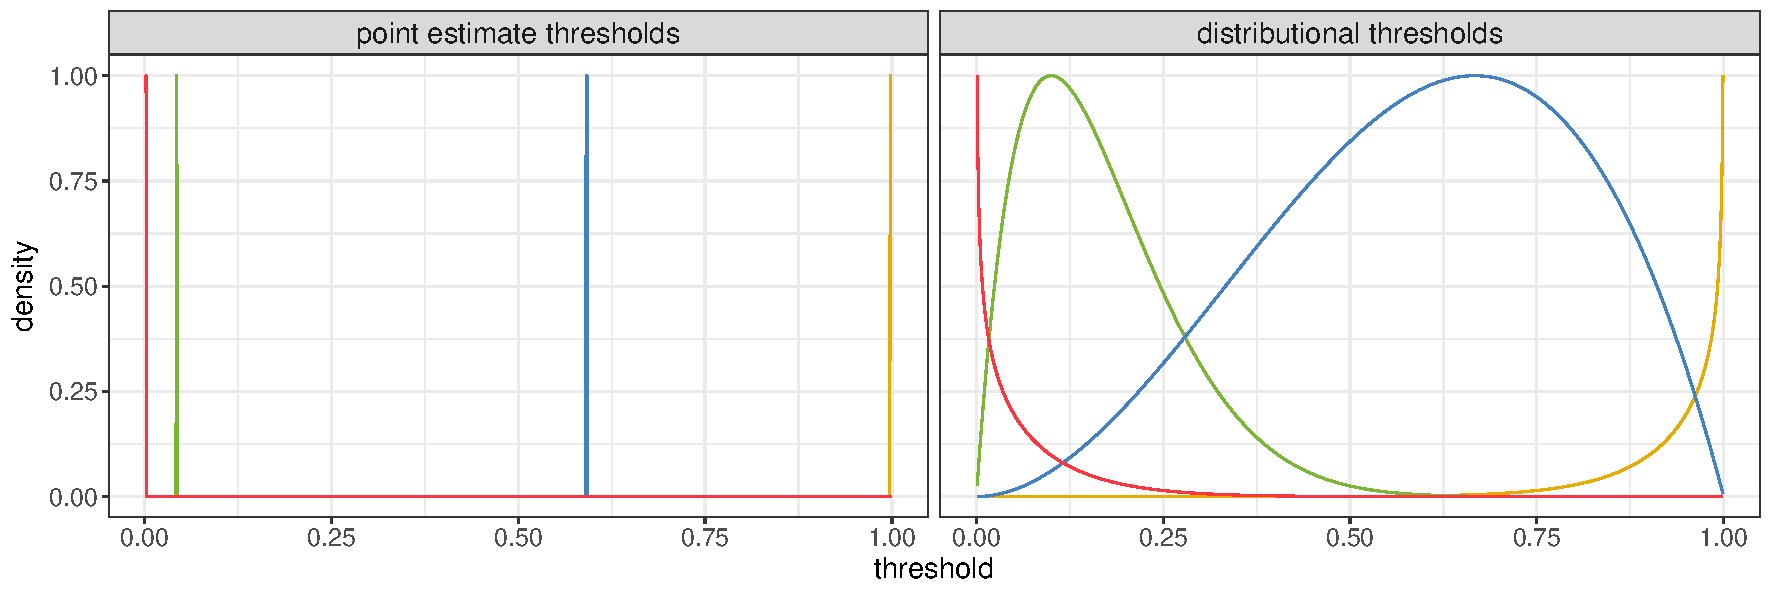
\includegraphics[width=\textwidth]{plots/fig-5a-model-visualization-distributions.pdf}

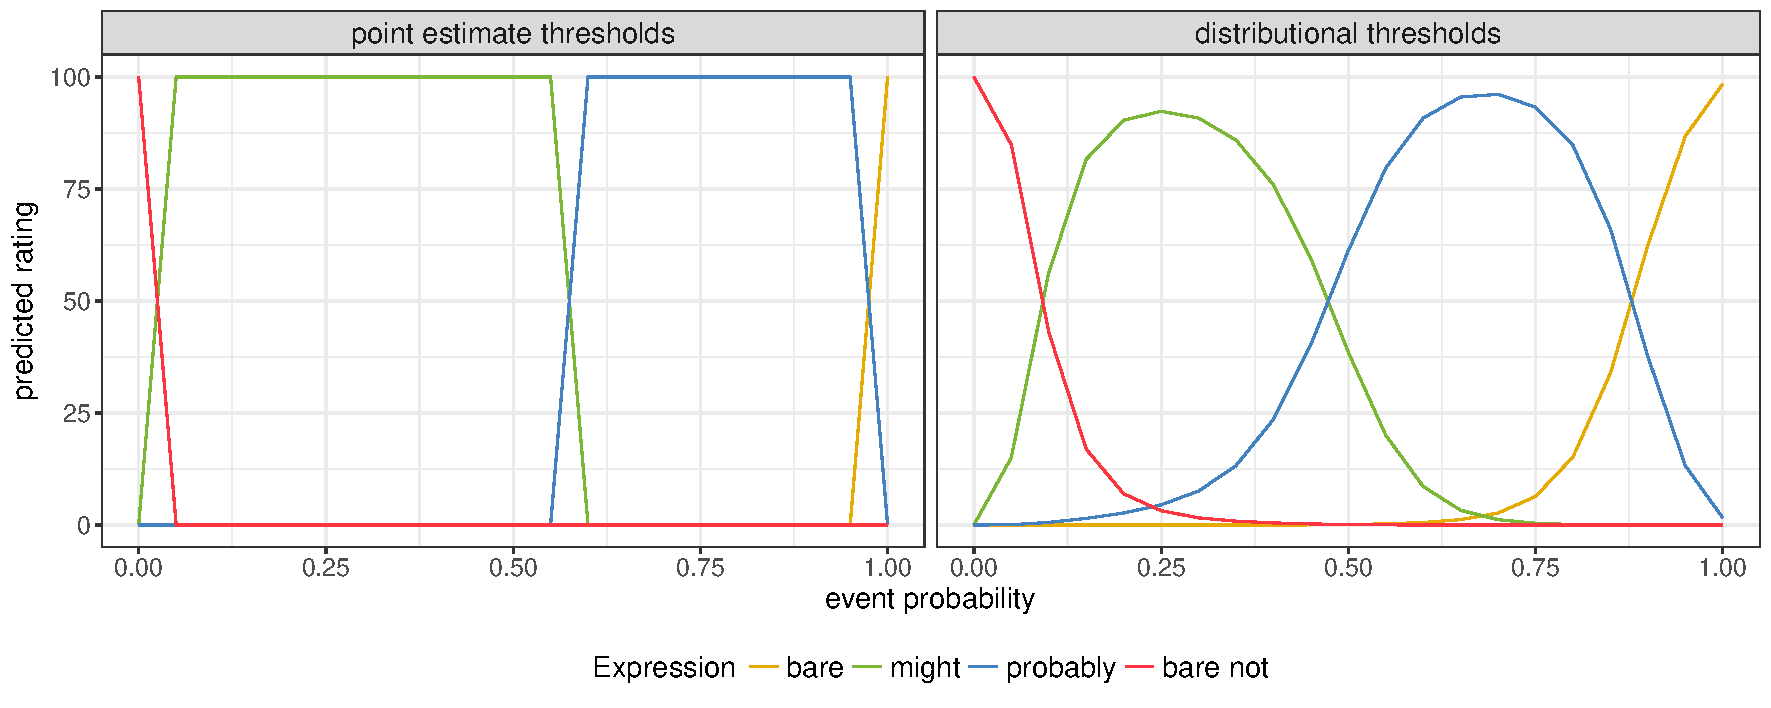
\includegraphics[width=\textwidth]{plots/fig-5b-model-visualization-predictions.pdf}

\caption{Example threshold distributions (upper panels) and corresponding model predictions for the \textit{expected pragmatic speaker} model (lower panels). In this example, the set of possible utterances is $U=\{$\textsc{bare}, \textsc{might}, \textsc{probably}, \textsc{bare not}$\}$, all utterances have equal costs, the rationality parameter $\lambda$ is set to 10, and the prior probability over event probabilities $P(\phi)$ is a uniform distribution. As the panels on the left show, point estimates of thresholds lead to sharp categorical boundaries in the model predictions, whereas distributions over thresholds, as in the panels on the right, lead to gradually increasing and decreasing predicted utterance ratings. \label{fig:model-visualization}}
\end{figure}

$S_1$ crucially depends on a vector of thresholds $\theta$ which contains a threshold for each uncertainty expression in the utterances in $U$, 
as well as a cost function $c(u)$. The values that participants expect a \textit{pragmatic speaker} to assign 
to these variables are unknown a priori; we infer these values from the data collected in the above reported experiment. 
In Experiment~1, we found that both at the population level and at the individual level, 
participants' ratings of the different expressions gradually increased and decreased with changing event probabilities 
(as, for example, shown in Figure~\ref{fig:norming-results-indiv}). This is expected if participants
have probabilistic beliefs about thresholds $\theta$ (as illustrated in the right panels of Figure~\ref{fig:model-visualization}) but not if they reason based on point estimates of $\theta$ (as illustrated in the left panels of Figure~\ref{fig:model-visualization}).
Considering these observations,  we assume that listeners hold beliefs about a speaker's thresholds in the form of a distribution $P\left(\theta_e\right)$.\footnote{We leave it open 
whether a {speaker} samples from a distribution over thresholds when producing utterances (as suggested by \cite{Qing2015}) 
or always uses the same values for thresholds. In the former case, listeners could have higher-order beliefs  $P(\eta)$ 
about different {speakers}' threshold distributions instead of having direct beliefs about the thresholds that different 
{speakers} use. For our purposes, this distinction does not matter since we assume that listeners would marginalize over higher-order beliefs $P(\eta)$ such that  $P\left(\theta_e\right) = \int P\left(\eta\right) P\left(\theta_e \mid \eta\right) d\eta$ and we therefore take the simplest approach and directly model $P\left(\theta_e\right)$. } Analogously, we assume that  listeners also have beliefs $P(c)$ about the speaker model's cost function.
Using these two distributions, we can define the \textit{expected pragmatic speaker} model $ES_1\left(u_e \mid \phi \right)$ as follows:

$$ES_1\left(u_e \mid \phi \right) = \int P(c) \int_0^1 P(\theta) S_1\left(u _e\mid \phi, \theta, c\right) d\theta \  d c$$

This model predicts which utterance listeners with uncertainty about a speaker's thresholds and cost function would expect that {speaker} to use to describe different event probabilities. 
Intuitively, this model can be seen as a weighted average of different \textit{pragmatic speaker} models, where individual models differ in terms of thresholds and cost functions.  The weights of this average are determined by listeners' belief distributions over thresholds and costs. For example, if listeners believe that it is likely that a speaker uses a threshold $\theta_{probably}$ of 0.5, they will assign higher weight to speaker models
using this threshold than models using other thresholds. 

\subsection{Linking function}

We assume that in Experiment~1, participants, when asked to provide ratings for utterances, reasoned about a generic speaker's 
likely descriptions of varying event probabilities. 
We assume that this reasoning was guided by participants' beliefs about the speaker's thresholds and costs, and 
that participants averaged over their uncertainty. For this reason, we assume that the population-level 
average ratings of what participants expect the speaker to say in different situations 
correspond to the probabilities predicted by the \textit{expected pragmatic speaker} model (with the \textit{something else}
option being predicted by the sum of the probabilities of all utterances not present in a condition; see below for more details).
Further, given the forced choice nature of the experiment and that we estimate model 
parameters from limited and potentially noisy data, we make the following additional linking assumptions
for which we provide a rationale and an assessment of their importance in turn.

\begin{itemize}
\item \textbf{Set of utterances}: Across all conditions, we assume that the set of utterances that participants are 
considering is the set of all utterances that we used in Experiment~1, i.e., $U= \{$ \textsc{bare}, \textsc{might}, 
\textsc{probably}, \textsc{think}, \textsc{looks like}, \textsc{could}, \textsc{bare not}$\}$. We include all utterances 
instead of only the utterances that are presented in a given condition since we assume that participants' general 
knowledge of English uncertainty expressions also influences their ratings. Ideally, we would include even more 
utterances in this set of alternatives but since we can only estimate parameters for uncertainty expressions for 
which we collected ratings, we are limited to the utterances in $U$. 

The exact set of utterances has only a small impact on the model's predictions as long as the set includes the \textsc{bare}
and \textsc{bare not} utterances as well as at least one utterance with a weaker 
(e.g., \textit{might}) and one with a stronger (e.g., \textit{probably})
uncertainty expression. If this requirement is met, the model makes the same qualitative predictions, 
and closely matches the quantitative predictions of a model that includes all 7 utterances choices.

\item \textbf{\textit{something else} option}: Participants in condition $\mathscr{C} = \{u_a, u_b\}$ 
could only choose between the three utterances $U' = \{u_a, u_b,$ \textit{something else}$\}$.
For modeling data from condition $\mathscr{C}$, we therefore need a function to predict the ratings 
for the utterances in $U'$. For $u_a$ and $u_b$, this is straightforward: We assume the probability 
of a participant choosing $u_a$ or $u_b$
is proportional to $ES_1(u_a \mid \phi)$ and $ES_1(u_b \mid \phi)$, respectively. 
We model the probability of a participant choosing the \textit{something else} option as the sum 
of the probability of all utterances that were not part of the condition as well as a constant $O$, 
which accounts for probability mass assigned to utterances that participants might be 
considering but which are not contained in $U$. This gives us the following condition-specific 
function $ES_1^{(\mathscr{C})}$ for predicting participants' ratings.

$$
ES_1^{(\mathscr{C})}(u \mid \phi) \propto 
    \begin{cases}
      ES_1(u \mid \phi) & \quad\mbox{if } u  \in \mathscr{C}\\
       O + \sum_{u \not \in \mathscr{C}} ES_1(u \mid \phi) & \quad \mbox{if $u$ is \textit{something else}} \\
   \end{cases}
$$

This summation over alternative utterances is crucial for fitting the data since we need to
capture the ratings for \textit{something else}. The only viable alternative would be
to fit individual curves for \textit{something else} for each condition, which would require
the estimation of considerably more parameters and would not explain the ratings for the
\textit{something else} option. The inclusion of the constant $O$ is less important but it
still improves model fit.


\item \textbf{Cost function}: We assume that the cost function represents participants' beliefs about the speaker's 
preferences for different utterances. Lower costs of an utterance indicate higher speaker preferences. We further 
assume that we are cueing participants to believe that the speaker would be likely to use the two utterances, $u_a$ 
and $u_b$, that are provided in condition $\mathscr{C}=\{u_a, u_b\}$ and that participants therefore primarily use the 
\textit{something else} option when both of the two utterances are semantically infelicitous or otherwise highly unexpected. 
We model this cueing effect in our choice of the cost function $c(u)$, which depends on the condition. For the two utterances 
that are presented to the participants, we set the cost to $1$ and for all the other utterances, we set the cost to a constant $\gamma > 1$:
$$
c(u, \mathscr{C}) = 
     \begin{cases}
       1 &\quad\text{if } u  \in \mathscr{C}\\
       \gamma &\quad\text{otherwise} \\
     \end{cases}
$$

Theoretically, we could have also used a different constant $\gamma_u$ for each utterance. The data from
Experiment~1, however, suggests that participants generally did not prefer one utterance over 
the other. To limit the number of free model parameters and to prevent overfitting, we therefore use a single
constant $\gamma$ for all utterances. We will, however, relax this assumption in our adaptation model in \sectionref{sec:model-adapt}, which
we use to investigate whether listeners update their beliefs about preferences during adaptation.

This condition-specific cost function is important for the model fit. If we didn't use such a cost function, 
the model would assign much higher ratings to the \textit{something else} option than participants did.

\item \textbf{Noise}: Finally, to account for participants not paying attention or making mistakes, 
we also include a noise term that models participants providing random ratings.
The amount of noise is captured by the noise strength parameter $\delta$. This parameter
indicates the proportion of random responses, that is, the proportion of responses drawn from a uniform distribution
over the three condition-specific responses $U'$. 

The inclusion of the noise term is not crucial for fitting the data but it does improve model fit and
is common practice in RSA models whose parameters are estimated from experimental data \cite[see][]{Herbstritt2019,Tessler2019}.

\end{itemize}

\noindent Incorporating all of these assumptions, we end up with the following noisy, condition-specific expected pragmatic speaker 
model $ES_1^{(\mathscr{C})'}(u \mid \phi)$, which we use to predict participants' ratings:

$$ES_1^{(\mathscr{C})'}(u \mid \phi) = \delta \times \frac{1}{|U'|} +  (1 - \delta) \times ES_1^{(\mathscr{C})}(u \mid \phi)$$

For the prior distribution over event probabilities $P(\phi)$, which is used in the literal listener model $L_0$, 
we use a uniform distribution over the interval $[0,1]$.\footnote{To 
verify the assumption that the prior on event probabilities is uniform, we conducted a separate norming study in which participants rated 
how likely they thought it was that a speaker described different gumball machines containing different 
proportions of blue and orange gumballs after hearing an unintelligible utterance. We found that on average 
participants rated all gumball machines equally likely which suggests that the prior over event probabilities is 
indeed uniform.} For the distributions over thresholds $P(\theta_e)$, we use a Beta distribution parametrized by 
$\alpha_e$ and $\beta_e$. The choice of Beta distributions is motivated by two of its properties. First, the support of a Beta distribution 
is the interval $[0,1]$ which corresponds to the exact range of possible values for $\theta_e$.

The second reason for using Beta distributions is that, depending on the parameterization, 
Beta distributions can take on very different shapes. This property is important because we are making
the simplifying assumption that all utterances in our experiments have a threshold semantics.
Such a semantics is commonly assumed for uncertainty expressions such as \textit{probably} \cite[e.g.,][]{Yalcin2010,Lassiter2016}, 
but it is unconventional for bare assertions such as \textit{``You'll get a blue one''}, which are generally assumed to be  
true only if the event is certain to happen, i.e., it has an event probability of 1. However, since Beta distributions can have a shape 
like the distribution for \textsc{bare} in the upper right panel in Figure~\ref{fig:model-visualization}, the model has the capability to infer
a semantics for the bare form that is almost equivalent to a traditional semantics of bare assertions. In this parameterization of the
Beta distribution, most probability mass is assigned to values of $\theta$ close to 1, which is mathematically almost equivalent to
a traditional semantics.\footnote{Alternatively, one can also see the threshold distribution for the bare form as a distribution over a verification parameter $\eta$ that governs 
how certain a speaker has to be to utter a bare assertion \cite[see, e.g.,][]{Lewis1976,Potts2007,Davis2007,Moss2018}. Mathematically, our assumption of bare forms having a threshold
semantics is equivalent to assuming that bare assertions are only true when a speaker's credence of the proposition exceeds the verification threshold $\eta$.}
Therefore, using Beta distributions for the threshold distributions has the desirable effect of allowing us a unified treatment of all expressions included in the model. 

\subsection{Parameter estimation}

Given all the assumptions outlined above, the model has  $18$ parameters in total: A cost parameter $\gamma$, a rationality parameter $\lambda$, a noise strength parameter $\delta$, a constant corresponding to other utterances $O$, and for each utterance, Beta distribution parameters $\alpha_e$ and $\beta_e$. We estimated these parameters jointly from all 21 conditions of Experiment~1 using Bayesian data analysis \cite[BDA; see, e.g.,][]{Kruschke2015}. To construct the dataset, we treated the ratings by each participant as a probability distribution from which we sampled 10 utterances. We used highly uninformative
uniform priors over the interval $[0,15]$ for the Beta distribution and cost parameters, uniform priors over the interval $[0,7]$ for the rationality parameter, and uniform priors over the interval $[0,0.5]$ for $O$ and the noise strength parameter. We estimated the vector of parameters $\Theta$ using MCMC with a Metropolis Hastings sampler. To decrease autocorrelation of the chain, we collected a sample only at every 10th iteration (i.e., we use thinning of 10). We discarded the first 10,000 burn-in samples and then collected 50,000 samples.  We ran four MCMC chains and confirmed convergence by computing the $\hat{R}$-statistic \cite{Gelman2003}. More details on the implementation of the model can be found in Appendix C.

\subsection{Model evaluation}

% Figure 6: plots/fig-6-pre_test_model_main.pdf (2-column figure)
\begin{figure}[th!]
\includegraphics[width=\textwidth]{plots/fig-6-pre\string_test\string_model\string_main.pdf}
\caption{Model predictions and results from Experiment~1. Error bars correspond to 95\% high density intervals (model predictions) and bootstrapped 95\%-confidence intervals (observed results). \label{fig:norming-results-model-main}}
\end{figure}


The result of the parameter estimation procedure is a posterior distribution over parameters given the observed data $P(\Theta \mid D_{obs})$. We evaluated
 model fit by performing a posterior predictive check \cite[PPC;][]{Kruschke2015}. To this end, we took 10,000 samples of parameters $\Theta$ from the posterior distribution. For each sample, we computed the model predictions $ES_1^{(\mathscr{C})'}(u \mid \phi)$ parameterized by $\Theta$. We then compared the average model predictions to the
mean ratings that participants had provided in the pre-exposure experiments. We further computed the 95\% high density interval  \cite[HDI;][]{Kruschke2015} which reflects the ctertainty of the model
about its predictions.

Figure~\ref{fig:norming-results-model-main} shows the model predictions and the experimental data for three conditions 
(see Table~\ref{tbl:correlations} and Appendix~D for modeling results for all 21 conditions). As these plots show, the model
is able to capture almost the entire variance in participants' average ratings. Further, the 95\% HDIs are very small, which suggests
that the model is certain about its predictions. Both of these observations are also true for the model's predictions for all the other
conditions. For 19 of the 21 conditions, the $R^2$ value between the model predictions and the experimental data exceeds 0.9,
and for the remaining 2 conditions, the $R^2$ value exceeds 0.88. 

Most cases in which the model predictions and the experimental data deviate concern the ratings at the two extremes of the event probability space.
The model often underpredicts ratings for the \textit{something else} option when there is either a 0\% or a 100\% chance of 
getting a target color gumball. In these situations, participants presumably thought that {\sc bare} and {\sc bare not} are the most appropriate
utterances and therefore rate \textit{something else} highly unless we provide them with the {\sc bare} or {\sc bare not} options. The model predicts
this behavior to some extent but seems to assume that participants were cued more heavily towards the presented utterance options than they actually were.
This could be an indicator that we should revisit our unconventional approach of treating the bare forms like uncertainty expressions with a threshold semantics,
since the model would predict higher ratings for \textit{something else} at both ends of the scale if we assumed that the bare form and its negation were only true
in the cases of 100\% and 0\% event probabilities, respectively. 
However, for our purposes in this paper, the exact predictions about production choices for objectively certain events are not as important and hence
we decided against revising the assumption that all utterances in the model have a threshold semantics.

The comparably low $R^2$ for the \textit{probably-think} condition ($R^2=0.88$) stems
from the fact that participants disagreed on the ordering of these two expressions. This  
led to a bimodal distribution of average ratings (see the figure in Appendix~B) for \textsc{think}, which our population-level 
model cannot fully capture. This suggests that if we wanted to perfectly model participants' production expectations, we should
additionally model participant-level differences. However, since the ordering of \textit{probably} and \textit{think} is not of great relevance
for our investigation of adaptation to different uses of \textit{might} and \textit{probably}, we did not attempt to fit a more complex model
that can account for individual listener differences. 

One potential concern given the flexibility of the model is that it could be overfitting the data. 
This is unlikely considering that all parameters are shared across all conditions and thus we are estimating only 18 parameters to predict in total 567 data points 
(27 data points for each one of the 21 conditions). To nevertheless rule out the possibility of overfitting, we performed a leave-one-out cross-validation of
the model. For each condition $x$, we estimated a distribution over parameters $\Theta_x$ using the data from all conditions but $x$. We then
compared the model predictions of the model parametrized by $\Theta_x$ to participants' ratings in condition $x$. This way, the model has to predict
participant behavior which it has not observed during parameter estimation. Table~\ref{tbl:correlations} shows the $R^2$ values for participants's
ratings and model predictions for the model estimated from all conditions and the leave-one-out models.

% Table 1
\begin{table}[ht!]
\center
\begin{tabular}{l | c | c}
      Condition & $R^2$ (all data) & $R^2$ (leave-one-out) \\
      \midrule
          bare-might  &  0.992  & 0.988 \\
       bare-probably  &  0.978  & 0.976 \\
          bare-could  &  0.978  & 0.976 \\
     bare-looks like  &  0.927  & 0.896 \\
          bare-think  &  0.968  & 0.964 \\
      might-probably  &  0.964  & 0.954 \\
         might-could  &  0.921  & 0.910 \\
    might-looks like  &  0.934  & 0.918 \\
         might-think  &  0.946  & 0.934 \\
      probably-could  &  0.961  & 0.959 \\
 probably-looks like  &  0.944  & 0.931 \\
      probably-think  &  0.888  & 0.860 \\
    could-looks like  &  0.924  & 0.910 \\
         could-think  &  0.931  & 0.920 \\
    looks like-think  &  0.970  & 0.960 \\
       bare not-bare  &  0.894  & 0.848 \\
      bare not-might  &  0.968  & 0.958 \\
   bare not-probably  &  0.910  & 0.893 \\
      bare not-could  &  0.910  & 0.840 \\
 bare not-looks like  &  0.927  & 0.903 \\
      bare not-think  &  0.933  & 0.920 \\
\end{tabular}
\caption{$R^2$ values for experimental data and model predictions for model estimated from all data and for models estimated from all conditions except the predicted condition. \label{tbl:correlations}}
\end{table}


As this table shows, the $R^2$ values remain high\footnote{We only observed slightly bigger drops in correlations for the \textit{bare not-bare} and the \textit{bare not-could} conditions. In these conditions, we paired expressions that are a poor description for a large range of event likelihoods: \textsc{bare not} and \textsc{bare} are only expected to be good descriptions if the event probability is very low or very high, respectively, and the \textit{bare not-could} condition includes expressions of which neither are well suited to describe high event probabilities. As a result, participants in these conditions seemed to be more uncertain what to do which was reflected in several participants commenting in a post-experiment survey that they would have answered differently had there been better response options. Participants' ratings were therefore presumably more idiosyncratic, which made it harder for the model to predict ratings without having access to the data from these conditions.} even if we exclude the data on which the model is evaluated from the model's training data, 
which suggests that our proposed model indeed explains
participants' expectations of a generic speaker's uncertainty expressions. 

% Figure 7: plots/fig-7-threshold-distributions-prior.pdf  (1.5-column figure)
\begin{figure}[th!]
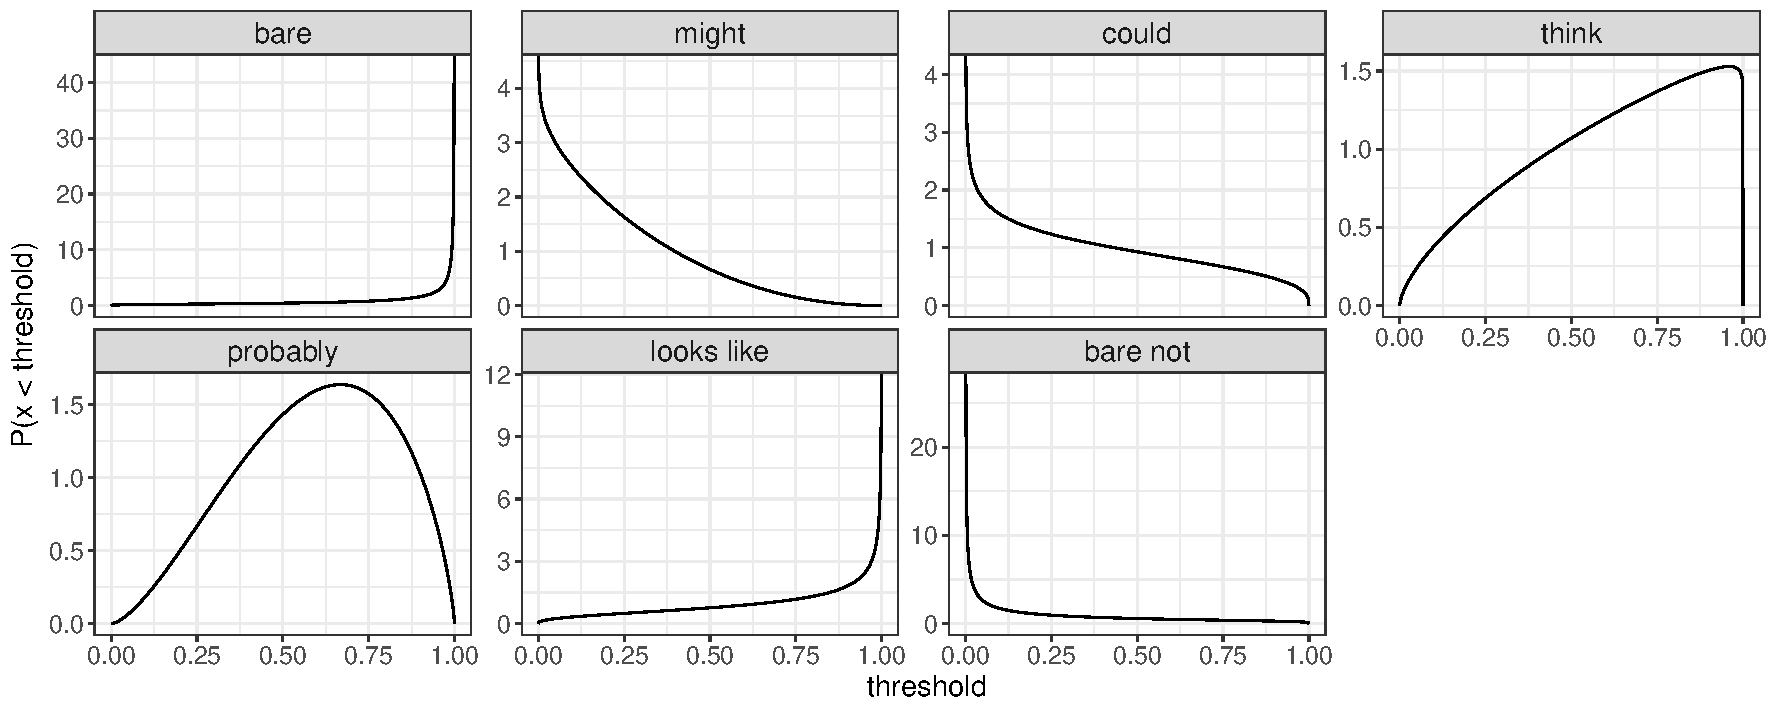
\includegraphics[width=\textwidth]{plots/fig-7-threshold-distributions-prior.pdf}
\caption{Inferred threshold distributions. For the negative bare utterance (\textsc{bare not}), the distribution is over an upper threshold, i.e., a bare statement embedded under negation is true if the probability of the event is lower than the threshold. For all other utterances, the distribution is over a lower threshold.
\label{fig:threshold-distributions}}
\end{figure}

Lastly, one of the advantages of Bayesian cognitive models is that their parameters are interpretable. Figure~\ref{fig:threshold-distributions} shows the 
maximum likelihood estimates of the inferred threshold distributions $P(\theta)$ for the seven uncertainty expressions that we included in our experiments.
The first observation is that most threshold distributions have considerable variance rather than being peaked at a particular value. This suggests that
listeners have probabilistic beliefs -- i.e., uncertainty -- about the semantic threshold for each utterance.

Further, the inferred threshold distributions are broadly in line with qualitative accounts of the meaning of uncertainty expressions.
As discussed above, for the bare form and its negation, we expected the model to infer threshold distributions whose probability mass is concentrated 
around $\theta=1$ and $\theta=0$, respectively.\footnote{Note that since the negation of the bare form is a negative form, $\theta$ is an upper threshold. For the bare form as well as
all the other utterances that we are are considering in this paper, $\theta$ is a lower threshold.} As  Figure~\ref{fig:threshold-distributions} shows, this is indeed what
the inferred threshold distributions look like. 

The probability mass of the threshold distribution for \textit{might} is  concentrated at values slightly above 0. This, too, 
is in line with non-probabilistic accounts of the interpretation of epistemic modals. These accounts generally assume that \textit{might} $p$ is true 
if there exists a world $w$ in a set of (contextually restricted) epistemically accessible worlds $E$ such that $p$ is true in $w$ 
\cite[e.g.,][]{Kratzer1991,Swanson2008,Hacquard2011}. One way to translate this logical condition into our probabilistic framework is to assume that 
in our gumball machine context, there exists an epistemically accessible world $w$ for each gumball $g$ and that in world $w$, one gets gumball $g$. 
Under this assumption, \textit{``You might get a blue gumball''} is true if there exists an epistemically accessible world $w$  in which one gets a
gumball $g$ that is blue. At the same time, if such a world exists, then $P(\mbox{blue gumball})$ is greater than 0, which approximately corresponds
to the threshold semantics with the inferred threshold distribution of the model. The inferred threshold distribution for \textit{could} is very similar, 
but not identical, to the one of \textit{might}. This also largely reflects the prediction by non-probabilistic accounts, which generally assume that \textit{might} and epistemic 
\textit{could} are semantically equivalent \cite{Kratzer1991,Hacquard2011}, but it also suggests that there are differences between these two expressions. 

The threshold distribution for \textit{probably} has most of its probability mass concentrated at thresholds above 0.5. This again largely reflects the predictions of 
existing accounts that assume that \textit{probably} $p$ is true if $p$ is more likely than the negation of $p$ \cite[e.g.,][]{Kratzer1991}. However, it is also noteworthy that the inferred
distribution has some probability mass below 0.5, which potentially provides evidence for theoretical arguments by \cite{Yalcin2010} that \textit{probably} $p$ can
sometimes also be true if $p$ is less likely than the negation of $p$.\footnote{Since we did not investigate whether participants always 
correctly perceived the event likelihood to be less than 0.5 for gumball machines with less than 50\% target color gumballs, an alternative explanation for this observation would be that participants sometimes overestimated the event likelihood and for this reason, they expected the generic speaker to use \textit{probably} despite an objective event likelihood of less than 0.5.}

The threshold distributions for the remaining expressions, \textit{looks like} and \textit{think} also match intuitions. The distribution for 
\textit{looks like} has most of its probability mass near threshold values of 1 but is overall slightly weaker, i.e., assigns higher probabilities to lower thresholds,
than the bare form. The distribution for \textit{think} assigns most probability mass to high thresholds, which is compatible with the intuition
that speakers use \textit{think} when they strongly believe the embedded proposition but are not entirely certain that it is true.
 
 
% Table 2
 \begin{table}[ht!]
\center
\begin{tabular}{l | c | c | c | c }
     & $\lambda$ (rationality) & $\gamma$ (cost) & $\delta$ (noise) & $O$ (other utterances) \\
      \midrule
      MAP & 2.21 & 3.03 & 0.074 & $3.64 \times 10^{-5}$ \\
      CI & [2.16, 2.26] & [2.98, 3.08] &  [0.069, 0.079] &[$2.89 \times 10^{-5}$, $4.50  \times 10^{-5}$] \\
         \end{tabular}
\caption{Estimated maximum a posteriori estimates (MAP) and 95\% credible intervals (CI) for model parameters. \label{tbl:model-params}}
\end{table}

\tableref{tbl:model-params} shows the MAP values and credible intervals for the remaining parameters. The model inferred that speakers
are relatively likely to choose an optimal utterance (reflected in the $\lambda$ parameter being
greater than 1); that utterances that are not included in the experiment incur a considerable cost  (reflected in the $\gamma$ parameter being greater than 1); that about 7.4\%
of the data should be treated as noise (reflected in the $\delta$ parameter); and that the production probability of utterances not included in our set of utterances is low. 

\subsection{Interim summary}

In this section, we described a computational model of production expectations of uncertainty expressions. This model
is couched within the RSA framework and assumes that listeners hold beliefs about a speaker's lexicon (in the form
of utterance-specific threshold distributions) and about speaker preferences (in the form of utterance-specific costs). We estimated 
the free parameters of this model from the results of Experiment~1, which resulted in a model that is able to accurately predict
participants' utterance ratings -- i.e., their expectations of use --  in Experiment~1 across all conditions with a shared set of parameters.

In the following sections of this paper, we will use this model as the basis for modeling adaptation. Since this model
is able to capture different beliefs about thresholds and preferences, it provides us with the opportunity to simulate 
the adaptation process as a result of updating beliefs about these model parameters. Further, in order to answer
our primary research question of whether listeners update their beliefs about lexica or preferences, we compare
different adaptation simulations in which we allow different types of parameters to be updated.

